\chapter{Camera Calibration in ATLASCAR 2}

One of the main tasks for this work was to develop and improve the ball detection fot the calibration package used previously by Silva \cite{VieiradaSilva2016} and Correia \cite{Correia2017}. In previous projects made with the ALTASCAR 2, the ball detection was done by only filtering the HSV values which was not enough to get optimal results.

\section{Implementation}

The ball detection upgrade begins by retrieving the video stream frames from the PointGrey camera. The image obtained was worked in a rosbag used for testing in order for the development to be made outside the ATLASCAR 2. The ball used in the tests is the ball in figure \ref{fig:ball}. 

\begin{figure}[htp]
	
	\centering
	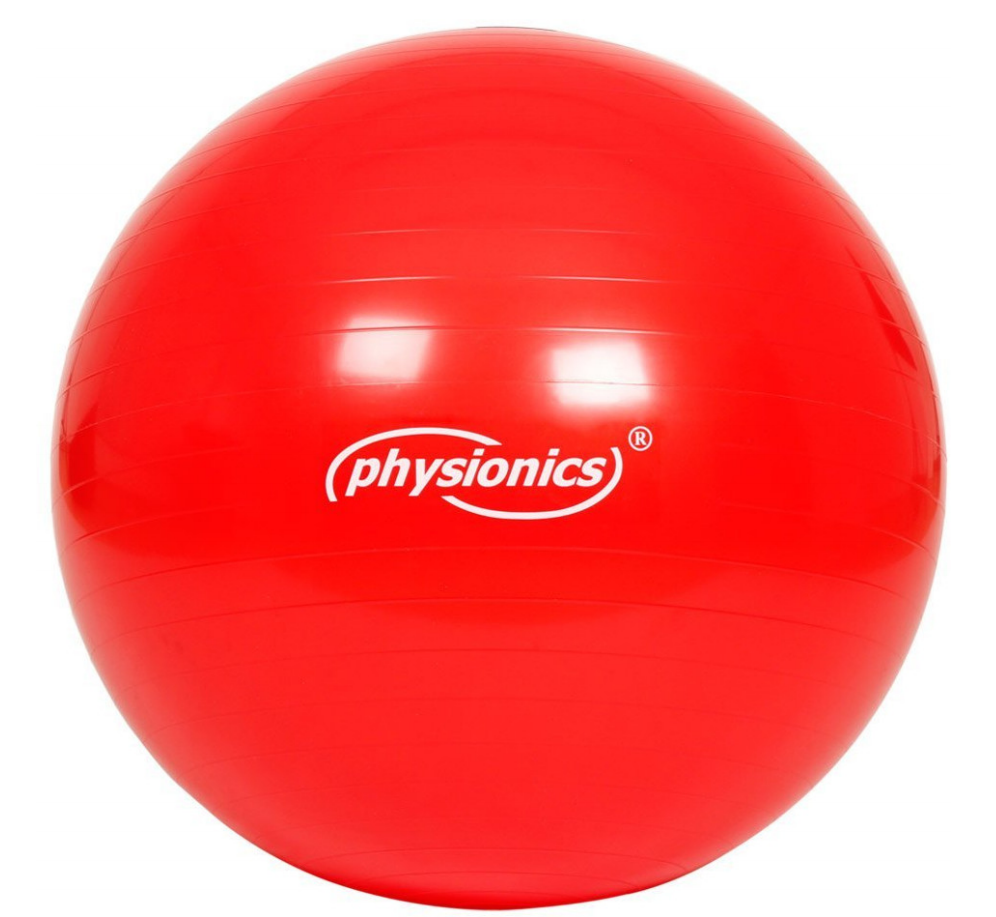
\includegraphics[width=0.4\textwidth]{capcalib/imgs/ball.png}
	
	\caption{Ball used for testing}
	\label{fig:ball}
	
\end{figure}

To acquire the images, the node creates a subscriber to get messages from the camera topic. ROS subscribers take the message in the topic and send it to a callback function in order to it to be processed. After obtaining information from the camera's message, it is needed to convert the RGB values into the HSV color space so that the image can be easily manipulated.

\subsection{Background Subtraction}

The first thing to do with the frames is to apply background subtraction. When the capture starts, the first received frame will be default background. To update the background to the actual frame in the stream the user presses the SPACEBAR (see figure \ref{fig:background}). The background removal is a process used in many vision based applications with static cameras, in which a frame is captured and defined as the background of a sequence of images. Therefore, when an objects enters the scene, by subtracting the background with the actual frame it is possible to detect easily where the object is. \cite{OpenCV}

Technically, background subtraction extracts the foreground from the static background. Most times, the background is worked out and a Gaussian blur is often applied to it. By defining a threshold, when subtracting the foreground with the background it is obtained a value for each pixel. It this value is higher than the threshold then (probably) an object entered that area.

\begin{figure}[htp]
	
	\centering
	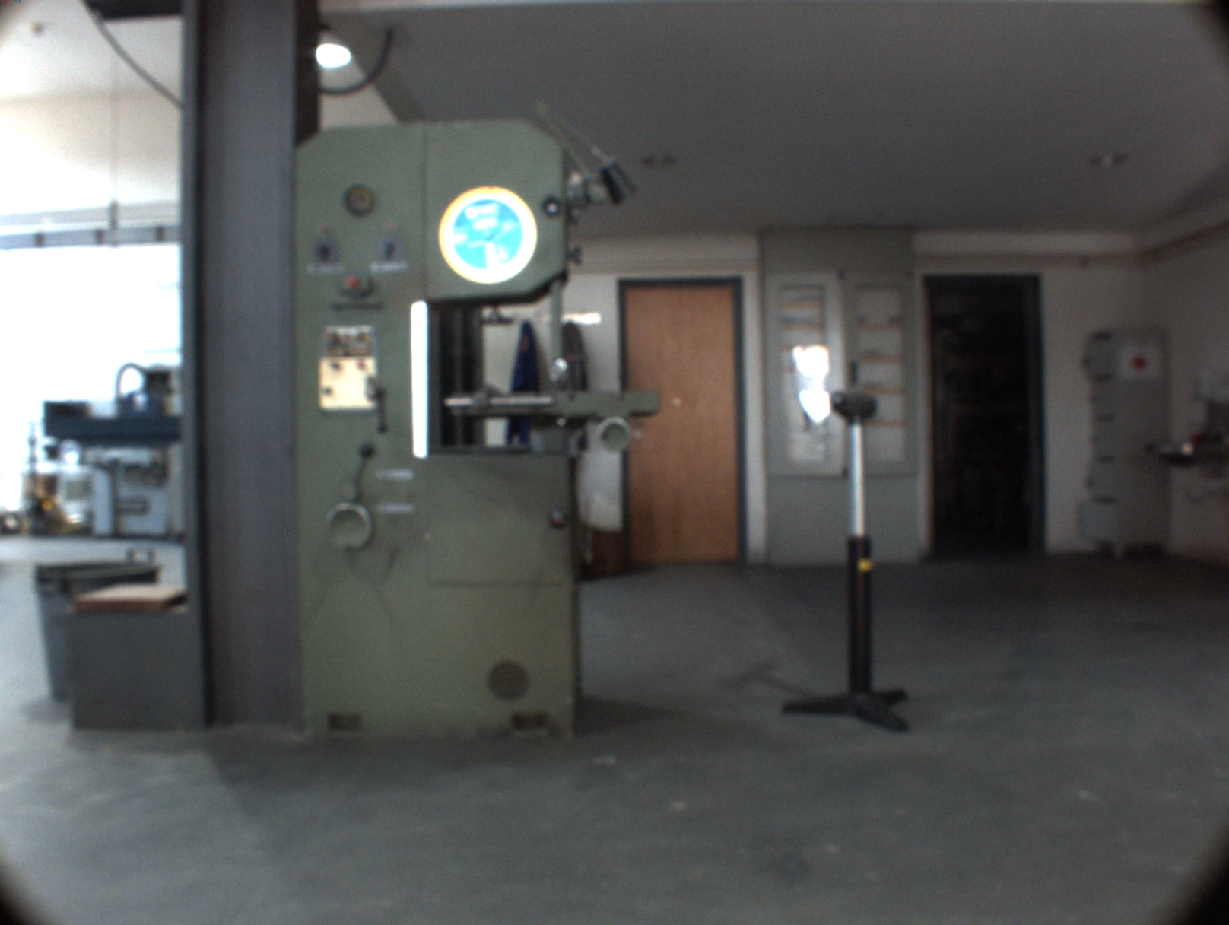
\includegraphics[width=0.7\textwidth]{capcalib/imgs/background.png}
	
	\caption{Background in test rosbag used for testing}
	\label{fig:background}
	
\end{figure}

The background removal process in the calibration package for the ball detection is done with applying blur to the background frame and then subtracting the background with the actual frame. This will result in a frame with very low values in the pixels where no new objects are shown. In most cases the values will not get to zero because of minor changes to the background which need to be ignored. A value is then used to apply a threshold in the resulting subtracted frame. If a pixel presents a value under the threshold, then it is set to zero (black), otherwise it is set to one (white). In the end, it is obtained a binary image containing some noise due to shadows or other lightning changes, and potentially an area with more concentrated white values where new objects appear. 


\begin{figure}[htp]
	
	\centering
	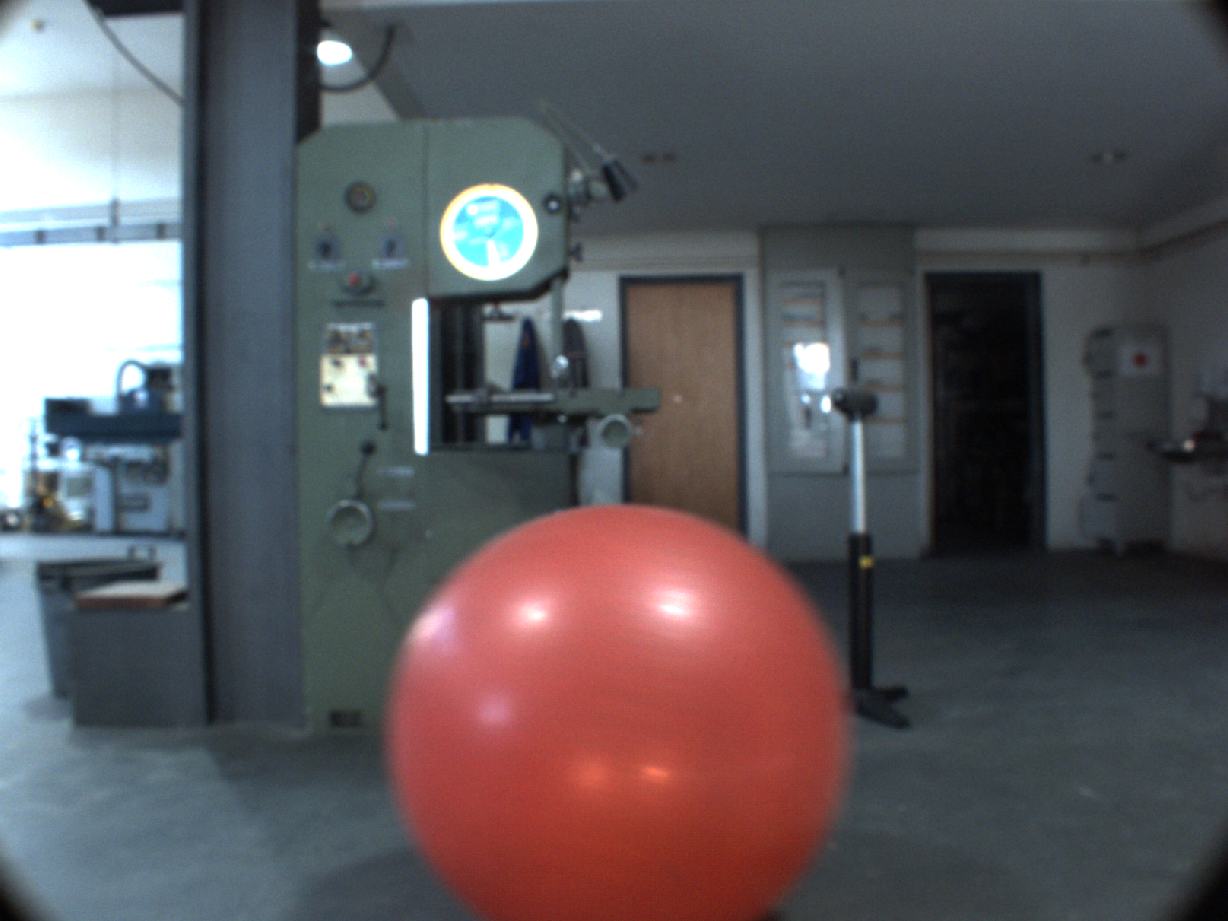
\includegraphics[width=0.7\textwidth]{capcalib/imgs/ball_test.png}
	
	\caption{Frame with ball rolling in front of the camera}
	\label{fig:balltest}
	
\end{figure}


\begin{figure}[htp]
	
	\centering
	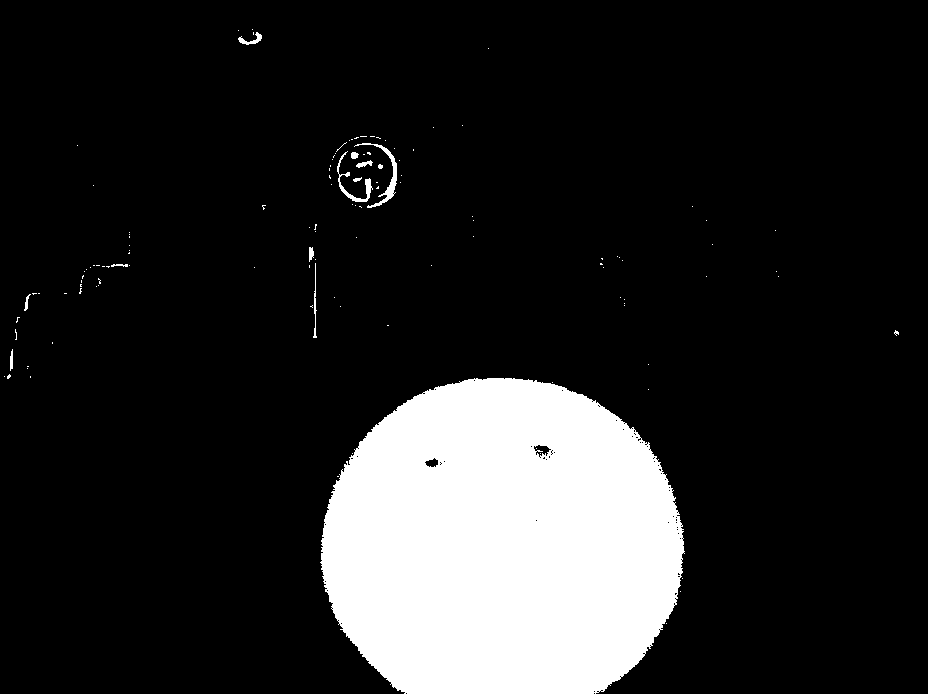
\includegraphics[width=0.7\textwidth]{capcalib/imgs/noise.png}
	
	\caption{Background subtraction result with noise}
	\label{fig:ballnoise}
	
\end{figure}

\subsection{Noise Filtering}

Assuming that the ball is rolling in the ground in front of the camera and that the car is leveled to the ground, it is possible to ignore the upper half of the image. All pixel in the upper half are then neglected and set to zero (black). Removing the upper half will then remove a major part of noise that can be created in the background.

To remove the rest of the noise in the lower half, the neighbor pixels are counted. The image is processed left-to-right, top-to-bottom, so the matrix corresponding to the frame is iterated throughout its lines. A counter is added to check if the previous pixels contained white pixels (pixels with value of 1). 

\begin{figure}[htp]
	
	\centering
	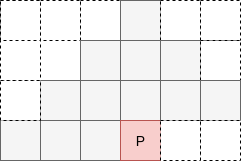
\includegraphics[width=0.5\textwidth]{capcalib/imgs/neighbor_count.png}
	
	\caption{Neighbor pixels used in the algorithm}
	\label{fig:neigh_cnt}
	
\end{figure}

The pixel in red with letter P in figure \ref{fig:neigh_cnt} represents the pixel being analyzed at the moment. If the pixel is black (zero) then it is not noise and nothing needs to be removed, but if the pixel is white (one) it is needed to look at the neighbor pixels. Around pixel P there are pixels with gray color. These are the pixels to be analyzed in the algorithm. The strategy is simple: if all of these pixels are set to one (white) the pixel P probably represents an object in the frame, but if one of the pixels is set to zero (black) then the pixel P is most likely to be a noise pixel and it is also set to zero.

This process is similar to what is called an erosion. Erosion is a morphological operations that consists in a set of operations that process images based on shapes applying a structuring element to an input image and generate an output image. In erosion, the algorithm computes a local minimum over the area of a kernel. In figure \ref{fig:neigh_cnt} the kernel is composed by the gray pixels. As the kernel is scanned over the image, the algorithm computes the minimal pixel value overlapped by the kernel and replaces the image pixel under the anchor point with that minimal value. \cite{OpenCV2.4.13.6documentation} 

\subsection{Color Filtering}

After the erosion is done, the ball in the image is beginning to be extracted. The next step is to separate the ball using color filtering. To set the ball color the user needs to click in the ball to capture its hue. A mouse event is triggered and an handler function is called. The handler localizes the mouse click and retrieves the RGB values of the pixel in those coordinates. These values are converted to a hue value of the HSV color space. The selected hue is the color used to filter the ball from the rest of the image. By applying certain thresholds it is possible to define an interval of color. The image will then be filtered by an interval centered in that hue value and the ball is now filtered from the rest of the image. 

A bounding box is drawn around the ball. To draw this box it is needed to calculate the ball center point and box upper-left point. The bounding box will only be drawn in the binary image if there is an area of white pixels big enough. To do this, the image is iterated like in this erosion phase, left-to-right and top-to-bottom. The algorithm saves the coordinates of all white pixels. An average $x$ and $y$ are calculated, finding the ball center. The size of the bounding box is given by how much white is in an specific area. Supposing there is a possibility of a white pixel to appear as noise, that pixel will have low weight in the algorithm considering that the pixels around it are black. Therefore, white pixels gathered in a larger area have high weight. Hence, the width and height of the bounding box are given by the maximum distance between the pixels with higher weight.


\begin{figure}[htp]
	
	\centering
	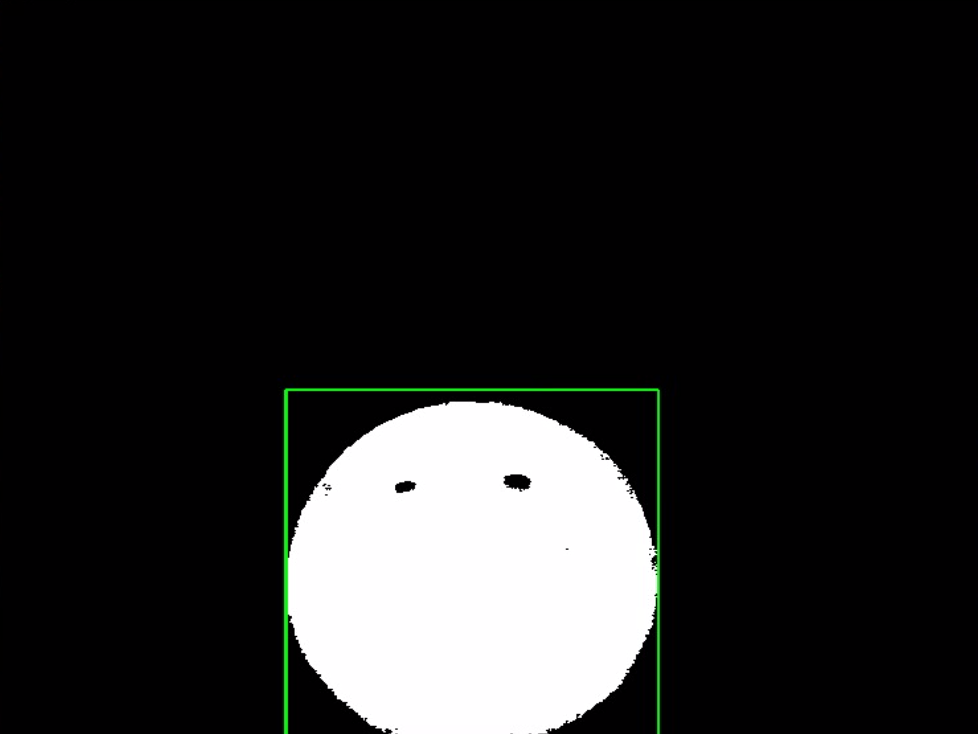
\includegraphics[width=0.7\textwidth]{capcalib/imgs/ball_detect.png}
	
	\caption{Ball detected with bounding box}
	\label{fig:balldetect}
	
\end{figure}

\subsection{Modifying the calibration package}

The calibration package used to calibrate the several sensors in ALTASCAR 2 uses multiple nodes, one for each kind of sensor. The camera node in the package is called \texttt{point\_grey\_camera} and it uses the source file \texttt{point\_grey\_camera.cpp}. This file was modified in order to add the implemented features into the calibration package. 

The \texttt{point\_grey\_camera} node receives the camera image by subscribing to the camera topic with ROS. The camera sends images in a ROS message format to be interpreted and processed by a callback function. The image processing algorithm follows the steps explained before in this section. After performing the ball detection, the center of the bounding box matching the center of the ball is retrieved. The ball center is published into the calibration package main node \texttt{calibration\_gui}.

To publish the ball center, a Canny image is retrieved from the binary image. The Canny algorithm is often used in visual computation applications to detect the edges of an object with low error rate, good localization and minimal response. OpenCV implements this function optimally by filtering any noise in the image using Gaussian filters. \cite{OpenCV2.4.13.6documentationa} Then it finds the intensity gradient of the image with a procedure analogous to Sobel. The Sobel derivatives uses discrete differentiation operators that compute an approximation of the gradient of an image intensity function combining Gaussian smoothing and differentiation. \cite{OpenCV2.4.13.6documentationb} 

With this, all pixel that are not considered to be part of an edge are removed and only thin lines (the edges) will remain. An upper and lower threshold is applied. This is called the hysteresis procedure and it consists in removing the pixels with a gradient below to the lower threshold. If the pixel has a gradient higher than the upper threshold then it is accepted as part of an edge.

The next step is to find the contours in the image edges. OpenCV implements a function for structural analysis and shape descriptors called \texttt{findContours}. The method retrieves contours from the binary image using the algorithm of Suzuki, S. and Abe, K. \cite{Suzuki1985}. The algorithm performs a point-in-contour test determining whether the point is inside a contour, outside, or lies on an edge. 

When the contours are found, it is needed to find to centroid of the ball. The radius of the ball is calculated with the size of the given bounding box. The real radius of the ball is passed as an argument so it is possible to calculate the distance from the camera to it. The centroids are obtained with a method based on the circle radius and they are published as \texttt{PointStamped} ROS points to be presented in the calibration GUI. 

\section{Results}

In figure \ref{fig:gui} the multisensor calibration GUI is shown with a test result. The SICK LMS151 LIDARS were used as point of reference for the purpose of demonstration and to have a comparator point to the camera.
\begin{figure}[htp]
	
	\centering
	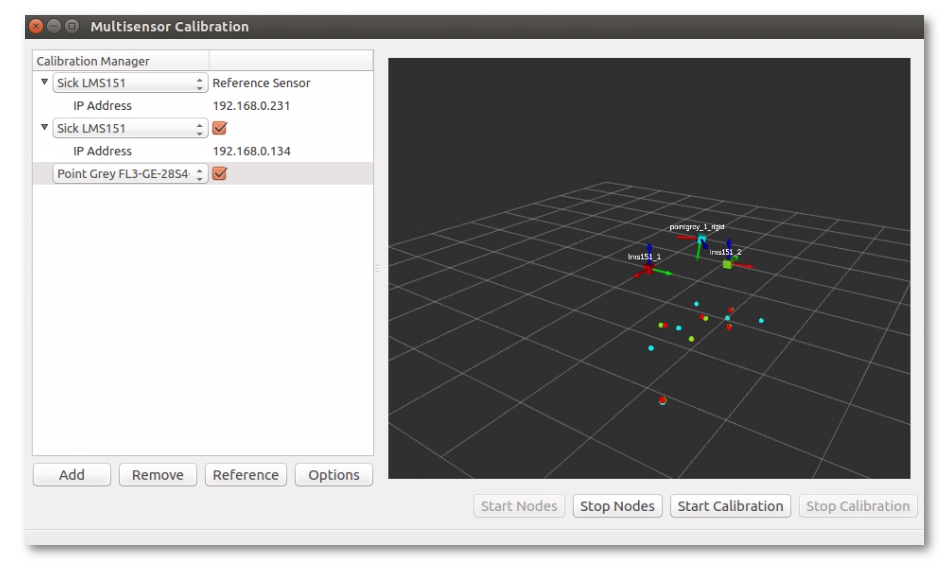
\includegraphics[width=0.9\textwidth]{capcalib/imgs/gui.png}
	
	\caption{Calibration GUI with calibration result}
	\label{fig:gui}
	
\end{figure}

During the calibration procedure, the ball rolls in front of the camera and sensors. The rage based sensors and the camera obtain a pointcloud of centroids of the ball during this activity. In the end, the transforms for each sensor are calculated, aligning the pointclouds of the several devices with each other. 

\begin{figure}
	\begin{center}
		\begin{lstlisting}[label={lst:calib_result}, caption={Calibration output file.},language=c++]
					-0.0563334  -0.998402 0.00440481   -1.07636
					  0.997797 -0.0561436  0.0353294    1.08224
					-0.0350256 0.00638533   0.999366  0.0617893
					         0          0          0          1	\end{lstlisting}
	\end{center}
\end{figure}

In listing \ref{lst:calib_result} an example output file of the calibration can be observed. The file contains a 4x4 matrix that indicates the transforms for the given sensor. Each sensor in the calibration will output its own file containing the transformation matrix. The reference sensor does not create a transform because it is assumed that this sensor is in the origin, unrotated. 



















 

